\documentclass{standalone}
\usepackage{tikz}
\usetikzlibrary{arrows,positioning,calc}
\usetikzlibrary{chains}
\usetikzlibrary{shapes.multipart}
\usetikzlibrary{shapes}
\begin{document}

\newsavebox{\task}
\savebox{\task}{%
    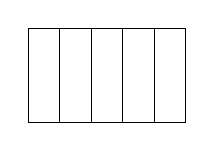
\begin{tikzpicture}[font=\small,
            >=stealth,
        ]
    \tikzset{every node/.style={rectangle split, draw, rotate=90}, rectangle split parts=5}
    \node[rectangle split, minimum width= 1.2cm,
                        minimum height = 1cm]  {};
    \end{tikzpicture}%
}

\begin{tikzpicture}
    {[start chain]
        \node[ellipse, start chain, minimum width=90pt, draw] (t1){\usebox{\task}};
        \node[ellipse, on chain, right=1cm of t1, draw] (t2) {\usebox{\task}};
        %\node[block,on chain,join=by {arrow},right=1cm of N1] (N2) {N2};
        \node[ellipse,on chain,right=1cm of t2, draw] (t3) {\usebox{\task}};
        \node[ellipse,on chain, right=1cm of t3] (t4) {$\cdots$};
        \node[ellipse,on chain,right=1cm of t4, draw] (t5) {\usebox{\task}};
    }
    % Arrows
     \path (t1) edge[very thick,->,bend left=30] node [left] {} (t2);
     \path (t2) edge[very thick,->,bend left=30] node [left] {} (t3);
     \path (t3) edge[very thick, ->,bend left=30] node [left] {} (t4);
     \path (t4) edge[very thick, ->,bend left=30] node [left] {} (t5);
     
    % Arrows
     \path (t5) edge[very thick, ->,bend left=30] node [left] {} (t4);
     \path (t4) edge[very thick, ->,bend left=30] node [left] {} (t3);
     \path (t3) edge[very thick, ->,bend left=30] node [left] {} (t2);
     \path (t2) edge[very thick, ->,bend left=30] node [left] {} (t1);
\end{tikzpicture}

\end{document}